\section{Results}\label{sec:results}

% auto-generated by make_arxiv_tables.py -- do not edit
\begin{table*}[t]\centering\small
\setlength{\tabcolsep}{3.5pt}
\caption{\textbf{Strict linear probe across task types} (balanced accuracy). Frozen encoder,
mean-pooled tokens, logistic regression with $C$ selected on the validation split, test scored
once; every model sees the identical samples and splits in its own input convention
(Sec.~\ref{sec:lpproto}), and every number is measured by us with the publicly released
weights. Every model is one checkpoint: SpecBraM is our main released checkpoint, the
baselines are their released ones. Brackets: 95\% confidence interval from 1{,}000 bootstrap
resamples of the test subjects (TUEV: recordings); the spread over our three pretraining seeds
is given in Appendix~\ref{app:fullmetrics}. REVE: readout selected on the validation split. BIOT's
released channel tokens cover only the sleep montage. Per-dataset results with Cohen's $\kappa$,
weighted F1 and AUROC/AUC-PR: Appendix~\ref{app:fullmetrics}. Bold: best per column.}
\label{tab:overview}
\resizebox{\textwidth}{!}{%
\begin{tabular}{l c cc cc c c c c}
\toprule
& & \multicolumn{2}{c}{Sleep staging} & \multicolumn{2}{c}{Clinical EEG} & \multicolumn{1}{c}{Workload} & \multicolumn{1}{c}{Depression} & \multicolumn{1}{c}{Emotion} & \multicolumn{1}{c}{Motor imagery}\\
\cmidrule(lr){3-4}\cmidrule(lr){5-6}\cmidrule(lr){7-7}\cmidrule(lr){8-8}\cmidrule(lr){9-9}\cmidrule(lr){10-10}
Model & Pretraining & ISRUC & HMC & TUAB & TUEV & MA & Mumtaz & FACED & PhysioNet-MI\\
\midrule
\textbf{SpecBraM} & $2{,}388$\,h & \ci{0.790}{0.764}{0.816} & \ci{\textbf{0.742}}{0.699}{0.776} & \ci{0.813}{0.775}{0.850} & \ci{0.555}{0.491}{0.648} & \ci{\textbf{0.781}}{0.722}{0.840} & \ci{\textbf{0.939}}{0.868}{0.995} & \ci{\textbf{0.221}}{0.195}{0.248} & \ci{\textbf{0.417}}{0.384}{0.450} \\
CBraMod & ${\sim}9$k\,h & \ci{0.728}{0.702}{0.752} & \ci{0.619}{0.576}{0.654} & \ci{0.778}{0.738}{0.814} & \ci{0.525}{0.471}{0.609} & \ci{0.653}{0.507}{0.799} & \ci{0.893}{0.760}{0.988} & \ci{0.171}{0.156}{0.188} & \ci{0.312}{0.286}{0.340} \\
LaBraM-Base & ${\sim}2.5$k\,h & \ci{0.752}{0.720}{0.777} & \ci{0.632}{0.583}{0.673} & \ci{0.776}{0.740}{0.812} & \ci{0.468}{0.416}{0.545} & \ci{0.681}{0.597}{0.736} & \ci{0.876}{0.744}{0.986} & \ci{0.167}{0.152}{0.181} & \ci{0.299}{0.285}{0.314} \\
BIOT & mixed & \ci{0.736}{0.691}{0.771} & \ci{0.658}{0.609}{0.697} & -- & -- & -- & -- & -- & -- \\
CSBrain & ${\sim}9$k\,h & \ci{0.730}{0.706}{0.752} & \ci{0.611}{0.580}{0.641} & \ci{0.772}{0.736}{0.805} & \ci{\textbf{0.564}}{0.505}{0.621} & \ci{0.556}{0.403}{0.653} & \ci{0.864}{0.774}{0.943} & \ci{0.179}{0.161}{0.199} & \ci{0.298}{0.273}{0.325} \\
REVE-Base & ${\sim}60$k\,h & \ci{\textbf{0.793}}{0.765}{0.816} & \ci{0.704}{0.664}{0.737} & \ci{\textbf{0.821}}{0.781}{0.861} & \ci{0.546}{0.500}{0.587} & \ci{0.684}{0.562}{0.771} & \ci{0.902}{0.743}{0.994} & \ci{0.200}{0.179}{0.225} & \ci{0.403}{0.371}{0.438} \\
\bottomrule
\end{tabular}}
\end{table*}


\subsection{Strict linear probe across tasks}\label{sec:lpfm}
Table~\ref{tab:overview} summarizes the strict linear probe on all tasks, grouped by task type.
As for the external models, which are released as single checkpoints, we evaluate one
checkpoint of SpecBraM, our main released model, and give every model a 95\% confidence
interval from 1{,}000 bootstrap resamples of the test subjects (TUEV: recordings). SpecBraM has
higher point estimates than CBraMod and LaBraM on every task, BIOT on sleep staging, and CSBrain
on every task except event classification (TUEV $0.555$ vs.\ $0.564$). REVE, of similar size but
pretrained on about 25 times more data, is the strongest baseline. On \emph{sleep staging}
SpecBraM has no detected difference on ISRUC ($0.790$ vs.\ $0.793$) and a higher point estimate on HMC ($0.742$ vs.\
$0.704$); on \emph{workload}, \emph{depression}, \emph{emotion} and \emph{motor imagery} its
point estimates are higher (mental arithmetic $0.781$ vs.\ $0.684$, Mumtaz $0.939$ vs.\ $0.902$, FACED $0.221$ vs.\
$0.200$, PhysioNet-MI $0.417$ vs.\ $0.403$); on \emph{clinical EEG} there is no detected
difference on event classification (TUEV $0.555$ vs.\ $0.546$), and its abnormality-detection point estimate is lower (TUAB $0.813$
vs.\ $0.821$). The intervals are wide for the small cohorts (mental arithmetic has four test
subjects, Mumtaz eleven), and the TUH tasks share corpus provenance with TUEG; their patients
were not excluded from our pretraining. Table~\ref{tab:paired} reports nominal, unadjusted
paired bootstrap intervals for the differences (Appendix~\ref{app:fullmetrics}). Intervals
containing zero indicate no detected difference under this procedure, not equivalence.
Appendix~\ref{app:fullmetrics} reports Cohen's $\kappa$, weighted F1 and, for
binary tasks, AUROC and AUC-PR for every dataset, together with the mean and standard deviation
over our three pretraining seeds.

Model size, input convention and readout also differ between the models; varying each in turn
(Appendix~\ref{app:confounds}) does not close the gap to CBraMod and LaBraM. Although our focus
is frozen use, SpecBraM also fine-tunes well: with full fine-tuning on sleep staging it reaches
$0.818$/$0.770$ balanced accuracy on ISRUC/HMC, above the listed published point estimates of
CBraMod, CSBrain and REVE under their respective recipes (Appendix~\ref{app:fttasks}).

\IfFileExists{tables/compute.tex}{% auto-generated by make_arxiv_tables.py -- do not edit
\begin{table}[t]\centering\small
\caption{\textbf{Along pretraining} (linear patch embedding, seed 42, strict linear probe BA;
bold: better target at that epoch).}
\label{tab:compute}
\begin{tabular}{c cc cc}
\toprule
& \multicolumn{2}{c}{ISRUC} & \multicolumn{2}{c}{HMC}\\
\cmidrule(lr){2-3}\cmidrule(lr){4-5}
Epoch & BP & Raw & BP & Raw\\
\midrule
1 & \textbf{0.7716} & 0.7398 & \textbf{0.7125} & 0.6593 \\
2 & \textbf{0.7812} & 0.7411 & \textbf{0.7222} & 0.6664 \\
4 & \textbf{0.7866} & 0.7431 & \textbf{0.7276} & 0.6689 \\
8 & \textbf{0.7904} & 0.7572 & \textbf{0.7477} & 0.7140 \\
12 & \textbf{0.7904} & 0.7688 & \textbf{0.7364} & 0.7160 \\
16 & \textbf{0.7901} & 0.7627 & \textbf{0.7420} & 0.7152 \\
\bottomrule
\end{tabular}
\end{table}
}{}
\IfFileExists{tables/target_r2.tex}{% auto-generated by make_arxiv_tables.py -- do not edit
\begin{table}[t]\centering\small
\caption{\textbf{How much of its pretraining target each model predicts}: fraction of the
target variance explained, $R^2=1-\mathrm{MSE}/\mathrm{Var}$, on the masked patches of 4{,}000
held-out windows (TUAB evaluation split, not excluded from TUEG pretraining; masks as in
pretraining), along pretraining (seed 42) and at the end over three seeds.
BP: mean of the five per-band $R^2$ values; waveform: pooled-sample $R^2$.
These are achieved scores, not estimates of Bayes ceilings. Band power, per band
$\delta/\theta/\alpha/\beta/\gamma$ at epoch 16: 0.89 / 0.89 / 0.92 / 0.94 / 0.95.}
\label{tab:target_r2}
\setlength{\tabcolsep}{6pt}
\begin{tabular}{l cc}
\toprule
Epoch & Band power & Raw waveform\\
\midrule
1 & 0.801 & 0.012 \\
2 & 0.880 & 0.016 \\
4 & 0.902 & 0.021 \\
8 & 0.909 & 0.025 \\
12 & 0.916 & 0.028 \\
16 & 0.917 & 0.031 \\
\midrule
16, three seeds & \val{0.917}{0.001} & \val{0.030}{0.000} \\
\bottomrule
\end{tabular}
\end{table}
}{}
% auto-generated by make_arxiv_tables.py -- do not edit
\begin{table}[t]\centering\small
\setlength{\tabcolsep}{3pt}
\caption{\textbf{Label efficiency} (strict linear probe, balanced accuracy vs.\ fraction of
labelled training epochs; ${<}100\%$: mean of five fixed random subsets shared by all
models). SpecBraM: main checkpoint. Bold: best per column.}
\label{tab:labeleff}
\resizebox{\columnwidth}{!}{%
\begin{tabular}{l cccccc}
\toprule
Model & 1\% & 5\% & 10\% & 25\% & 50\% & 100\%\\
\midrule
\multicolumn{7}{l}{\emph{ISRUC}}\\
BIOT & 0.655 & 0.703 & 0.716 & 0.728 & 0.734 & 0.736 \\
CBraMod & 0.660 & 0.709 & 0.717 & 0.726 & 0.727 & 0.729 \\
LaBraM-Base & 0.680 & 0.724 & 0.730 & 0.741 & 0.746 & 0.752 \\
CSBrain & 0.633 & 0.693 & 0.708 & 0.721 & 0.726 & 0.730 \\
REVE-Base & 0.736 & 0.771 & 0.778 & 0.788 & \textbf{0.791} & \textbf{0.792} \\
\textbf{SpecBraM} & \textbf{0.760} & \textbf{0.779} & \textbf{0.788} & \textbf{0.791} & \textbf{0.791} & 0.790 \\
\multicolumn{7}{l}{\emph{HMC}}\\
BIOT & 0.582 & 0.625 & 0.638 & 0.648 & 0.655 & 0.658 \\
CBraMod & 0.539 & 0.590 & 0.602 & 0.613 & 0.616 & 0.620 \\
LaBraM-Base & 0.574 & 0.616 & 0.621 & 0.630 & 0.631 & 0.633 \\
CSBrain & 0.509 & 0.581 & 0.595 & 0.608 & 0.612 & 0.612 \\
REVE-Base & 0.635 & 0.679 & 0.691 & 0.700 & 0.702 & 0.704 \\
\textbf{SpecBraM} & \textbf{0.662} & \textbf{0.698} & \textbf{0.717} & \textbf{0.733} & \textbf{0.738} & \textbf{0.742} \\
\bottomrule
\end{tabular}}
\end{table}


\begin{figure}[t]\centering
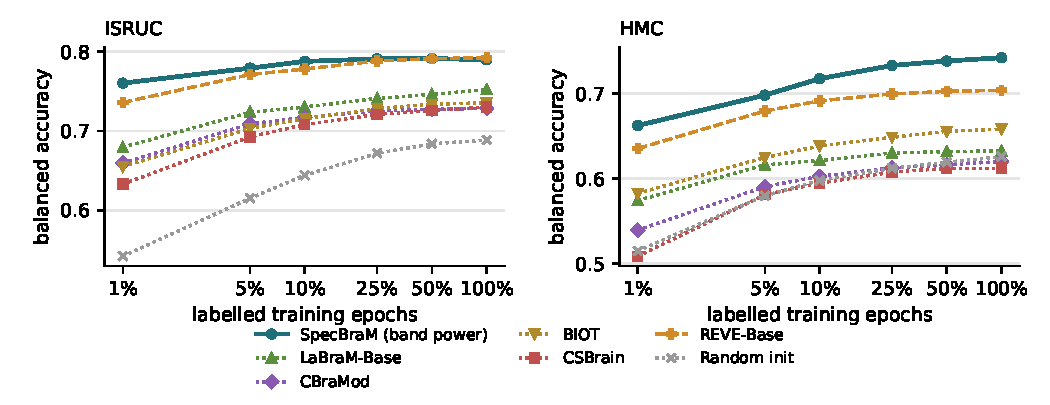
\includegraphics[width=\columnwidth]{figures/label_efficiency_lp.pdf}
\caption{\textbf{Label efficiency} under the strict linear probe (balanced accuracy;
SpecBraM: main checkpoint).}
\label{fig:labeleff}
\end{figure}

% auto-generated by make_arxiv_tables.py -- do not edit
\begin{table}[t]\centering\small
\setlength{\tabcolsep}{3.5pt}
\caption{\textbf{Clustering evaluation}: k-means ($k{=}5$) on frozen sleep features of the
test split (standardized, 64 PCA dimensions; cluster fitting uses no labels), agreement with the
expert stages. Mean over five k-means seeds; our rows: seed-42 checkpoints.
REVE: readout selected by validation NMI using labels. Bold: best per column.}
\label{tab:cluster}
\resizebox{\columnwidth}{!}{%
\begin{tabular}{l cc cc}
\toprule
& \multicolumn{2}{c}{ISRUC} & \multicolumn{2}{c}{HMC}\\
\cmidrule(lr){2-3}\cmidrule(lr){4-5}
Model & NMI & ARI & NMI & ARI\\
\midrule
\textbf{SpecBraM} & \textbf{0.417} & \textbf{0.310} & \textbf{0.236} & \textbf{0.179} \\
Raw-waveform recon.\ (same arch.) & 0.401 & 0.278 & 0.182 & 0.135 \\
\midrule
CBraMod & 0.277 & 0.184 & 0.083 & 0.056 \\
LaBraM-Base & 0.356 & 0.291 & 0.083 & 0.051 \\
BIOT & 0.149 & 0.091 & 0.057 & 0.025 \\
CSBrain & 0.263 & 0.166 & 0.069 & 0.038 \\
REVE-Base & 0.323 & 0.279 & 0.155 & 0.103 \\
\bottomrule
\end{tabular}}
\end{table}


\subsection{Efficiency}\label{sec:efficiency}
\noindent\textbf{Pretraining steps.} Table~\ref{tab:compute} follows the linear probe along
pretraining for the two targets, with everything else fixed. After a single epoch, band power
reaches $0.772$ on ISRUC, above raw-waveform reconstruction after sixteen epochs ($0.763$); on
HMC it is close after one epoch ($0.713$ vs.\ $0.715$) and exceeds it after two ($0.722$).
Band power thus reaches the final quality of waveform reconstruction with 8 to 16 times fewer
pretraining steps (P2). Target computation uses one FFT per
patch, the head has five outputs per patch instead of 200, no tokenizer is trained beforehand
(as for LaBraM) and no target network is maintained (as for latent prediction).

\noindent\textbf{Achieved target prediction.} Table~\ref{tab:target_r2} measures prediction
on TUAB evaluation windows with the masks of pretraining. These windows are held out from
downstream training; exclusion from pretraining is not established. The
band-power model explains $80\%$ of its target's variance after one epoch and $92\%$ after
sixteen; the waveform model explains $1.2\%$ after one epoch and $3.1\%$ after sixteen. Band-power
$R^2$ is averaged over the five per-band scores, whereas waveform $R^2$ pools the sample
coordinates. These are achieved scores, not Bayes predictability ceilings: residual error
combines contextual uncertainty with model and optimization error, and does not determine a
fraction of gradient noise. The early improvement of band-power prediction accompanies the
early rise of its linear probe.

\noindent\textbf{Model size and data.} At 4.2M parameters, the size of CBraMod, the band-power
model ($0.788$/$0.728$ on ISRUC/HMC) surpasses the 51.3M-parameter waveform model
($0.770$/$0.715$; Table~\ref{tab:ablation}), and it exceeds CBraMod, pretrained on about four
times more data, by $6.0$/$10.9$ points. SpecBraM is pretrained on $2{,}388$ hours, about a
quarter of the data of CBraMod and CSBrain and a twenty-fifth of REVE's, and ranks first on
most tasks of Table~\ref{tab:overview}.

\noindent\textbf{Labels.} On sleep staging, SpecBraM remains effective with few labelled
training epochs (Table~\ref{tab:labeleff}, Fig.~\ref{fig:labeleff}). With $1\%$ of the training epochs SpecBraM
reaches $0.760$/$0.662$ on ISRUC/HMC, more than BIOT, CBraMod, LaBraM and CSBrain obtain with all
labels, and against $0.736$/$0.635$ for REVE with $1\%$. It approaches REVE's full-training-label score
with $25\%$ of the training epochs on ISRUC ($0.791$ vs.\ $0.792$) and exceeds it with $10\%$ on HMC
($0.717$ vs.\ $0.704$), and on HMC it leads every external model at every label fraction.

\noindent\textbf{Unsupervised clustering.} To assess the representation without a supervised classifier,
we cluster the frozen sleep features with k-means and compare the clusters with the expert
stages (Table~\ref{tab:cluster}). SpecBraM's features are organized by sleep stage more than
those of any other model: NMI $0.417$/$0.236$, against $0.401$/$0.182$ for the same-architecture
raw-reconstruction model and at most $0.356$/$0.155$ for the external models. These results
support sleep-stage structure in the frozen features. Clustering is unsupervised, but REVE's
readout is selected by validation NMI using stage labels; this comparison is therefore not
entirely label-free.

% auto-generated by make_arxiv_tables.py -- do not edit
\begin{table*}[t]\centering\small
\setlength{\tabcolsep}{4pt}
\caption{\textbf{Pretext-target study} at matched backbone, data ($2{,}388$\,h), steps (16
epochs) and launcher; only the target (or the tokenizer) changes. Strict linear probe,
mean${\pm}$std over three pretraining seeds unless stated. ``1\%'': balanced accuracy with
$1\%$ of the labelled training epochs (mean of five fixed subsets). $\Delta$: difference to the
band-power row of the same block, in balanced-accuracy points; paired by pretraining seed, band
power exceeds raw-waveform reconstruction on every seed in every block. Bold: best per column.}
\label{tab:ablation}
\begin{tabular}{l cc cc cc}
\toprule
& \multicolumn{2}{c}{BA (100\% labels)} & \multicolumn{2}{c}{BA (1\% labels)} & \multicolumn{2}{c}{$\Delta$ BA (pts)}\\
\cmidrule(lr){2-3}\cmidrule(lr){4-5}\cmidrule(lr){6-7}
Target & ISRUC & HMC & ISRUC & HMC & ISRUC & HMC\\
\midrule
\multicolumn{7}{l}{\emph{Linear patch embedding, 51.3M parameters (main model)}}\\
\textbf{Band power} (ours) & \val{\textbf{0.7965}}{0.0059} & \val{\textbf{0.7433}}{0.0019} & \val{\textbf{0.765}}{0.006} & \val{\textbf{0.670}}{0.008} & -- & -- \\
Raw-waveform reconstruction & \val{0.7701}{0.0076} & \val{0.7153}{0.0028} & \val{0.721}{0.017} & \val{0.617}{0.017} & -2.6 & -2.8 \\
\midrule
\multicolumn{7}{l}{\emph{Linear patch embedding, 4.2M parameters (CBraMod's size)}}\\
Band power (ours) & \val{0.7882}{0.0053} & \val{0.7284}{0.0040} & \val{0.741}{0.021} & \val{\textbf{0.670}}{0.012} & -- & -- \\
Raw-waveform reconstruction & \val{0.7537}{0.0042} & \val{0.6738}{0.0083} & \val{0.709}{0.008} & \val{0.607}{0.002} & -3.5 & -5.5 \\
\midrule
\multicolumn{7}{l}{\emph{Filterbank tokenizer}}\\
Band power (ours) & \val{0.7961}{0.0067} & \val{0.7371}{0.0059} & \val{0.764}{0.003} & \val{0.658}{0.016} & -- & -- \\
Raw-waveform reconstruction & \val{0.7716}{0.0058} & \val{0.7201}{0.0087} & \val{0.707}{0.026} & \val{0.623}{0.008} & -2.5 & -1.7 \\
Band-waveform reconstruction & \val{0.7646}{0.0063} & \val{0.7173}{0.0026} & \val{0.695}{0.013} & \val{0.622}{0.006} & -3.2 & -2.0 \\
\bottomrule
\end{tabular}
\end{table*}


\subsection{Controlled target study}\label{sec:targetstudy}
Table~\ref{tab:ablation} changes only the pretext target, with backbone, data, steps and
launcher fixed, and reports the mean over three pretraining seeds. With the linear patch
embedding the band-power target reaches $0.7965$/$0.7433$ balanced accuracy on ISRUC/HMC, against
$0.7701$/$0.7153$ for raw-waveform reconstruction (P1). The difference is $+2.6$/$+2.8$ points with the linear embedding,
$+2.5$/$+1.7$ with a learnable filterbank tokenizer and $+3.5$/$+5.5$ at 4.2M parameters;
paired by pretraining seed, it is positive on all eighteen seed--dataset pairs, and it grows to
$+3.2$ to $+6.3$ points with $1\%$ of the labels. Reconstructing five band-pass-filtered
waveforms instead of the raw one gives lower mean scores ($0.7646$/$0.7173$ vs.\ $0.7716$/$0.7201$; P3).
This is consistent with benefits from an aggregated, phase-invariant target, but does not
isolate phase removal: output dimension and loss scale also change. Beyond sleep, band power
has higher mean scores on mental arithmetic, depression screening and event classification,
and close scores on the other tasks (Appendix~\ref{app:targettasks}). Both studied spectral
estimators give strong sleep results (Appendix~\ref{app:variants}).
